\documentclass{article}
\usepackage{tikz}
\usetikzlibrary{angles, quotes}
\usepackage{amssymb}
\usepackage{pgfplots}
\pgfplotsset{width=10cm,compat=1.9}
\usepgfplotslibrary{statistics}
\usepackage[left=2.54cm,right=2.54cm,top=2.54cm,bottom=2.54cm]{geometry}
\usepackage{tasks} %Paquete necesario para la producción de items horizontales para algunos ejercicios de tarea empleando el comando /begin{multicols}}{#}.../end{multicols} para ayudarnos a reducir las páginas
\usepackage{pdflscape} %comando que permite cambiar a orientación horizontal las hojas%
\usepackage{soul} %Paquete para permitir la compilación de acentos usando el comando {\hl{}}}\\
\sethlcolor{yellow(munsell)} %comando para definir el color para el subrayado usando el comando \hl
\usepackage[utf8]{inputenc}
\usepackage[spanish]{babel}
\usepackage{icomma}
\usepackage{ragged2e}
\usepackage{siunitx}
\usepackage{url}
\usepackage[colorlinks=true, urlcolor=blue,  linkcolor=black, citecolor=green]{hyperref}
\usepackage{pdfpages}
\usepackage{blindtext} %Paquete que genera texto ficticio (dummy text) con el comando: \blindtext
\usepackage{cancel} %in the preamble gives you four different modes of striking through: \cancel{text to cancel} draws a diagonal line (slash) through its argument, \bcancel{text to cancel} uses the negative slope (a backslash), \xcancel{text to cancel} draws an X (actually \cancel plus \bcancel), \cancelto{〈value〉}{〈expression〉} draws a diagonal arrow through the 〈expression〉pointing to the 〈value〉 (math-mode only)
\usepackage{csquotes}
\usepackage{afterpage}
\usepackage{parskip} 
\usepackage{float}
\usepackage{enumitem}
\usepackage{multicol}%Paquete que permite la creación aislada de columnas de texto. De esta forma se reduce la cantidad de páginas en nuestro documento
\usepackage{lipsum} %Paquete que genera texto de relleno al igual que \usepackage{blindtext}, se usa con el comando \lipsum[#-#] los #(hashtags) delimitan el número de páginas que deseamos ocupar del paquete lipsum para usarlos como relleno. 

% Definir el comando personalizado para la nota
\newcommand{\mynote}[1]{%
\begin{tikzpicture}[baseline=-0.75ex]
\node[draw, circle, fill=Apple Green!60, inner sep=2pt] (note) {\textbf{Nota:}};
\end{tikzpicture}%
\ \textit{#1}%
}

\newenvironment{Figura}
{\par\medskip\noindent\minipage{\linewidth}}
{\endminipage\par\medskip}
\usepackage{caption}
\usepackage[
backend=biber,
sorting=none,
url=true
]{biblatex} %bibliografía
\addbibresource{biblio.bib}
% Establecer el espacio entre las entradas de la bibliografía
\setlength{\bibitemsep}{1\baselineskip} % Puedes ajustar el valor según tus preferencias
\usepackage{amsmath,amsthm,amssymb,amsfonts}
\usepackage{pifont} %Permite la compilación del comando \xmark: es el símbolo de la tachita
\usepackage{mathtools} %permite la compilación de símbolos para matrices
\usepackage{empheq} %Paquete que se relaciona con \usepackage[most]{tcolorbox} para la creación de cuadros/cajas de colores para delimitar los resultados matemáticos o líneas de texto usando la línea de comando: \begin{empheq}[box={\mymath[colback=orange(webcolor)!70,drop lifted shadow]}]{equation*} \end{empheq}
\usepackage[most]{tcolorbox} %Paquete que se relaciona con \usepackage{empheq} para la creación de cuadros/cajas de colores para delimitar los resultados matemáticos o líneas de texto
\renewcommand{\qedsymbol}{$\blacksquare$}
\usetikzlibrary{positioning,decorations.pathreplacing} %Paquete que permite la compilación de llaves para cuadros sinópticos (brace diagram) 
\usepackage{schemata} %The schemata package is designed just for these brace diagrams
\usepackage{booktabs}

\newcommand\AB[2]{\schema{\schemabox{#1}}{\schemabox{#2}}} %comando o paquete necesario para crear cuadros sinópticos

\newtcbox{\mymath}[1][]{%
nobeforeafter, math upper, tcbox raise base,
enhanced, colframe=blue!30!black,
colback=blue!30, boxrule=1pt,
#1} %Comando importante para encasillar los resultados matemáticos en cajas de diferentes colores, se relaciona con los paquetes \usepackage{empheq} y \usepackage[most]{tcolorbox} 

\newenvironment{sysmatrix}[1]
{\left(\begin{array}{@{}#1@{}}}
{\end{array}\right)}
\newcommand{\ro}[1]{%
\xrightarrow{\mathmakebox[\rowidth]{#1}}%
}
\newlength{\rowidth}% row operation width
\AtBeginDocument{\setlength{\rowidth}{3em}}  %Comando importante para laproducción de lineas de operaciones entre matrices, método de Gauss o Gauss Jordan se relaciona con \newenvironment{sysmatrix}

%formato para cambiar el horario a español
\usepackage[spanish]{datetime2}
\DTMsetdatestyle{spanish}

\renewcommand{\today}{\DTMdisplaydate{\the\year}{\the\month}{\the\day }{-1}}
%%%%%%%%%%%%%%%%%%%%%%%%%%%%%%%%%%%%%%%%%

\usepackage{datetime}
\newcommand{\mycurrenttime}{\xxivtime}

%%%%%%%%%%%%%%%%%%%%%%%%%%%%%%%%%%%%%%%%%%%%%%%%%%%%%%%%%%%%%%%%%%%%%%%%%%%%%%%%%%%%%%%%%%%%%%%%%%%%%%%%%%%%%%%%%%%%%%%%%%%%%%%%%%%%%%%%%%%%%%%%%


%%%%%%%%%%%%%Caja de color para el título%%%%%%%%%%%%%%%%%%%%%%%%%%%%%%%%%%%%%%%%%%%%%%%%%%%%%%

\definecolor{myframecolor}{RGB}{1, 45, 75} % Prussian Blue
\definecolor{myboxcolor}{RGB}{0, 107, 92} % Apple Green

\newtcolorbox{mybox}{
enhanced,
colback=myboxcolor!7, % Color de fondo del cuadro
colframe=myframecolor, % Color del marco del cuadro
arc=0pt,
boxrule=1pt,
borderline west={2mm}{-10mm}{myframecolor}, % Borde en el lado izquierdo
sharp corners=southwest,
width=\linewidth,
before=\par\vspace{\bigskipamount}, % Espacio antes del cuadro
after=\par\vspace{\bigskipamount} % Espacio después del cuadro
}


\newcommand{\euler}{e} %Comando para producir letra e de euler
\newenvironment{remark}{\par\vfill\footnotesize % Vertical white space above the remark and smaller font size
\begin{list}{}{
	\leftmargin=80pt % Indentation on the left
	\rightmargin=60pt}\item\ignorespaces % Indentation on the right
\makebox[-2.5pt]{\begin{tikzpicture}[overlay]
		\node[draw=Horizon!60,line width=2.5pt,circle,fill=Horizon!25,font=\sffamily\bfseries,inner sep=4pt,outer sep=0pt] at (-19pt,5pt){\textcolor{Horizon}{Nota}};\end{tikzpicture}} % Blue Nota in a circle
\advance\baselineskip -1pt}{\end{list}\vskip5pt} % Tighter line spacing and white space after remark
\usepackage{graphicx}

\usepackage{titling}

\input{colores.tex}

%%Producir signos de cita textual``Asignatura''

\newcommand{\xmark}{\ding{55}} %%%comando que genera la tachita

\newenvironment{MyColorPar}[1]{%
\leavevmode\color{#1}\ignorespaces%
}{%
}%

%%%%%%%%%%%%%%%%%%% Título de la tarea, Nombre de alumno

\title{Tarea 1}
\author{\emph{Julio Alfredo Ballinas García} $\boldsymbol{\mid}$ 202107583}
\date{\today}

%%%%%%%%%%%%%%%%%%% Datos de la Materia

\usepackage{fancyhdr}
\fancypagestyle{plain}{%  the preset of fancyhdr 
\fancyhf{} % clear all header and footer fields
\fancyfoot[R]{
\includegraphics[width=2cm]{LogoFCFMBUAP (1).png}}
\fancyfoot[L]{{\bfseries{\thedate{}}} a las {\bfseries{\mycurrenttime{}}} horas{} (GMT-6, H. Puebla de Zaragoza, Pue)}
\fancyhead[L]{Escritura de textos científicos}
\fancyhead[R]{\theauthor}
}
\makeatletter
\def\@maketitle{%
\newpage
\null
\vskip 1em%
\begin{center}%
\let \footnote \thanks
{\LARGE \@title \par}%
\vskip 1em%
%{\large \@date}%
\end{center}%
\par
\vskip 1em}
\makeatother

\usepackage{lipsum}  
\usepackage{cmbright}


%%%%%%%%%%%%%%%%%%%%%%%%%%%%%%%%%%%%%%%%%%%%%%%%%%%%%%%%%%%%%%%%%%%%%%%%%%%%%%%%%%%%%%%%%%%%%%%%%%%%%%%%%%%%%%%%%%%%%%%%%%%%%%%%%%%%%%%%%%%%%%%%%%%%%%%%%%%%%%%%%%%%%%%%%%%%%%%%%%%%%%%%%%%%%%%%%%%%%%

\begin{document}



\maketitle


%%%%%%%%%%%%%%%%%%% Datos del profesor, campus y aula

\begin{mybox}
\noindent\begin{tabular}{@{}ll}
	{\bfseries{Profesor}} & Dra. Claudia Oliva Mendoza Barrera\\
	\textcolor{prussianblue}{\bfseries{Campus}} / \textcolor{trueblue}{\bfseries{Facultad}}  & \textcolor{prussianblue}{\bfseries{C.U. BUAP}} /  \textcolor{trueblue}{\bfseries{FCFM}} \\
	\textcolor{prussianblue}{\bfseries{Edificio}} /  \textcolor{trueblue}{\bfseries{Salón}}    & 	\textcolor{prussianblue}{\bfseries{EMA4}} /  \textcolor{trueblue}{\bfseries{409}}   
\end{tabular} 
\end{mybox} \vspace{1cm}

\section{Instrucciones de los ejercicios}
\addcontentsline{toc}{section}{Instrucciones de los ejercicios}

\setlength{\columnsep}{2cm}
\begin{multicols}{2} 
\begin{enumerate}[label={{\textcolor{trueblue}{\textbf{Ej}. \arabic*.0}}}, start=1]
	\item Realizar una búsqueda de tesis o tema de tesis en la base de datos.
	\begin{enumerate}
		\item \textbf{Web of Science (WOS)}
		\item \textbf{Google académico / Google Scholar}
		\item \textbf{Open Knowlede Maps}
		\item \textbf{Connected papers}
	\end{enumerate}
\end{enumerate}

\begin{enumerate}[label={{\textcolor{trueblue}{\textbf{Ej}. \arabic*.0}}}, start=2]
	\item Aprender a realizar búsquedas académicas propias.
\end{enumerate}  

\begin{enumerate}[label={{\textcolor{trueblue}{\textbf{Ej}. \arabic*.0}}}, start=3]
	\item Enviar la búsqueda realizada a \href{cmendoza@fcfm.buap.mx}{cmendoza@fcfm.buap.mx} antes del día jueves
\end{enumerate} 

\begin{enumerate}[label={{\textcolor{trueblue}{\textbf{Ej}. \arabic*.0}}}, start=4]
	\item Seleccionar \textbf{5 artículos} \underline{relevantes} sobre el tema de interés.
\end{enumerate} 

\begin{enumerate}[label={{\textcolor{trueblue}{\textbf{Ej}. \arabic*.0}}}, start=5]
	\item Entregar un documento (Word, {\LaTeX} \hspace{1mm} o  PDF)
	\begin{enumerate}
		\item Nombre del estudiante.
		\item Línea de investigación actual o deseada.
		\item Enlace de cada artículo.
		\item Síntesis breve (2 líneas) de cada artículo, revisando resumen y resultados.
	\end{enumerate}
\end{enumerate} 

\end{multicols} 

\tableofcontents \newpage

\begin{center}
\begin{tikzpicture}
	% Dibuja círculos rellenos en diferentes colores
	\fill[bittersweet] (0,0) circle (0.17cm);
	\fill[Apple Green] (0.6,0) circle (0.17cm);
	\fill[trueblue] (1.2,0) circle (0.17cm);
	\fill[Aguamarina] (1.8,0) circle (0.17cm);
	\fill[Sun] (2.4,0) circle (0.17cm);
	\fill[orange(colorwheel)] (3.0,0) circle (0.17cm);
	\fill[Pesto] (3.6,0) circle (0.17cm);
	\fill[blue-violet] (4.2,0) circle (0.17cm);
	\fill[ticklemepink] (4.8,0) circle (0.17cm);
	\fill[Gallery] (5.4,0) circle (0.17cm);
	\fill[Mantle] (6.0,0) circle (0.17cm);
	\fill[Nevada] (6.6,0) circle (0.17cm);
	\fill[onyx] (7.2,0) circle (0.17cm);
	% Agrega más círculos o modifica los colores según sea necesario
\end{tikzpicture}
\end{center}  \vspace{2cm}


\section{Nombre del alumno: Julio Alfredo Ballinas García} \vspace{0.5cm}

\subsection{\textcolor{Apple Green}{\textbf{Línea de investigación actual o deseada}}: Estudiar el \textcolor{Mahogany}{\textbf{\underline{café}}} de distintas regiones del país con la finalidad de caracterizar los compuestos presentes en cada una de las fases de producción y lograr obtener una buena calidad de grano.} \vspace{0.5cm}

\subsubsection{\textbf{Artículo 1:} \textcolor{Cinnabar}{\textbf{Glucosylated forms of serotonin and tryptophan in green coffee beans (2016) -  LWT - Food Science and Technology}}}  \vspace{0.5cm}

\textbf{Autores:} \textit{Servillo}, Luigi; \textit{Giovane}, Alfonso; \textit{Casale}, Rosario; \textit{Cautela}, Domenico; \textit{D$^{\prime}$Onofrio}, Nunzia; \textit{Balestrieri}, María Luisa; \textit{Domenico Castaldo}. \vspace{0.5cm}

\textbf{Resumen}:  En este estudio se propone estudiar la presencia de formas glucosadas de \underline{serotonina} y sus derivados \textbf{N-metilados} en granos de café verde de las especies \textbf{Robusta} ( \textit{Coffea canephora Pierre ex A. Froehner}) y \textbf{Arábica} (\textit{ Coffea arabica. L }). La serotonina es un neurotransmisor derivado del triptófano con roles fisiológicos importantes en humanos y plantas. Estudios previos ya habían detectado serotonina y melatonina en granos de café verde y tostado.  Los autores utilizan análisis \textbf{HPLC-ESI-MS2} para examinar los granos de café verde. \vspace{0.5cm}

\textbf{Resultados}: Este estudio reporta por primera vez la presencia de \textbf{serotonina $5-0-\beta-\text{glucósido}$} y \textbf{triptófano-N1-glucósido} en granos de café verde. \vspace{0.5cm}

\underline{Efectos del tostado}: Ni el \textbf{triptófano- N1-glucósido} ni la \textbf{serotonina $5-0-\beta-\text{glucósido}$}  fueron detectados en los granos de café tostado, lo que sugiere que el proceso de tostado degrada estos compuestos presentes naturalmente en los granos de café verde.

\underline{Triptófano-N1-glucósido como marcador de origen}: Existe una notable diferencia en los niveles de \textbf{triptófano-N1-glucósido} entre \textbf{Robusta} y \textbf{Arábica} convierte a este compuesto como una herramienta potencial para la autenticación del origen de los lotes de granos de café verde. \vspace{0.5cm}

\textbf{Enlace}: \href{https://webofscience.bibliotecabuap.elogim.com/wos/woscc/full-record/WOS:000381321100018}{WOS/artículo} \vspace{0.5cm}

\subsubsection{\textbf{Artículo 2:} \textcolor{trueblue}{\textbf{Measurement of caffeine in coffee beans with UV/vis spectrometer (2008) - Food Chemistry}}} \vspace{0.5cm}

\textbf{Autores}: \textit{Belay}, Abebe; \textit{Ture}, Kassahun; \textit{Redi}, Mesfin; \textit{Asfaw}, Araya. \vspace{0.5cm}


\textbf{Resumen}: En este estudio se utiliza espectroscopía Uv/vis para determinar la cantidad de cafeína en granos de café, los autores obtienen coeficientes de absorción molar decádica y momento dipolar de transición de la cafeína en los valores de $\lambda = 272 \, nm$ y $\lambda = 274.7 \, nm$, tanto para agua como para \underline{diclorometano}. Para lograr la extracción de la cafeina presente en el café disuelto en agua se utiliza \underline{diclorometano}, esto se hace ya que no es posible medir directamente la cafeína con el uso directo de UV/vis debido a la superposiicón espectral. Se utiliza también un \underline{ajuste gaussiano} para eliminar la posible interferencia en el espectro de la cafeína. \vspace{0.5cm}

\textbf{Resultados}: Se confirmó que no es posible medir directamente la cafeína de los granos mediante espectrofotometría UV/vis debido a la presencia de compuestos que absorben en la región UV y causan ruido. Se usa \underline{diclorometano} para la extracción de la cafeína y se observó que el ajuste gaussiano ayuda a eliminar interferencia de compuestos del ácido clorogénico que ensucian la muestra. Luego de aplicar el ajuste gaussiano, las métricas obtenidas de cafeína fueron idénticas al de la cafeína pura. \vspace{0.5cm}

Los resultados de este estudio son los siguientes:	\vspace{0.5cm}


\textbf{Caracterización de cafeína pura} \vspace{0.5cm}

\begin{enumerate}
	\item \textbf{Coeficientes de de absorción molar decádica de la cafeína}:  $1115 \, m^{2} mol^{-1}$ en \underline{agua} a $272 \, nm$ y $1010 \, m^{2} mol^{-1}$ en \underline{diclorometano} a $274\text{.}7 \, nm$ 
	\item \textbf{Valores calculados para el momento dipolar de transición}: $10\text{.}40 \times 10^{-30} Cm$ en \underline{agua} y $10\text{.}80 \times 10^{-30} Cm$ en \underline{diclorometano}.\\
	\item \textbf{Espectro de absorción UV-vis}: En \underline{agua} fue en la región de $243-302\, nm$ con un pico de absorbancia de $1\text{.}224$ en $\lambda =272 \, nm$, mientras que para la cafeína en \underline{diclorometano} fue en la región $243-301\, nm$ con un pico de absorbancia de $1\text{.}043$ en $\lambda =274\text{.}7 \, nm$
\end{enumerate} \vspace{0.5cm}

\begin{figure}[H]
	\centering
	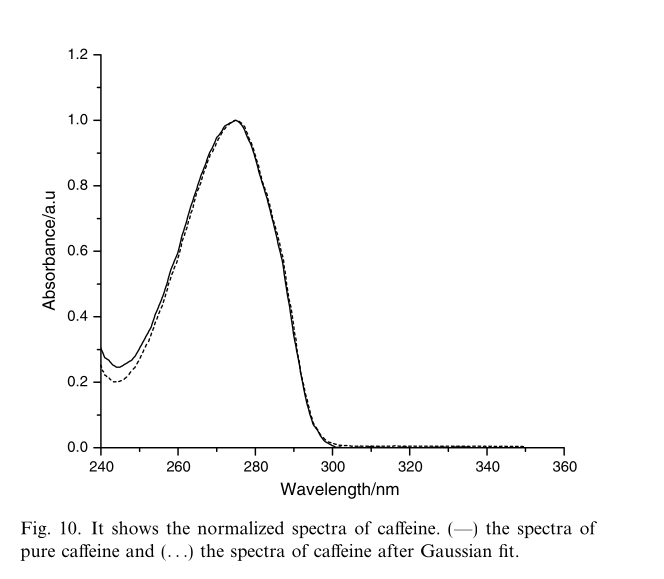
\includegraphics[width=0.8\textwidth]{images/absorbancia_cafeína.png}
	\caption{Resultados con ajuste gaussiano}
	\label{fig:ajuste-gaussiano}
\end{figure} \vspace{0.5cm}

\textbf{Enlace}: \vspace{0.5cm}

\href{https://www.connectedpapers.com/main/5135ae6a3d92e94d6bc22e4c8575d759a8763676/Measurement-of-caffeine-in-coffee-beans-with-UV%2Fvis-spectrometer/graph}{connectedpapers} \vspace{0.5cm}

\href{https://doi.org/10.1016/j.foodchem.2007.10.024}{DOI} \vspace{0.5cm}


\subsubsection{\textbf{Artículo 3:} \textcolor{Sun}{\textbf{Spectrophotometric analysis of caffeine (2021) - IOP Conference Series: Materials Science and Engineering}}} \vspace{0.5cm}

\textbf{Autores}: \textit{Misto}; \textit{Alawiyah}, K.; \textit{Rohman}, L.; \textit{Supriyadi}; \textit{Mutmainnah}; \textit{Purwandari}, E. \vspace{0.5cm}

\textbf{Resumen}:  En este estudio realizado en Jember, Indonesia se determina el contenido de cafeína en café Arábica puro local y mezclas de Arábica con maíz.  También se examinan cómo las diferentes temperaturas de tostado afecan el contenido de cafeína. El café es un producto de alto valor económico en Indonesia, y a la cafeína es un metabolito secundario presente naturalmente en muchas plantas. La cafeína es un compuesto orgánico con nitrógeno, del grupo de las metilaxinas, cuya fórmula química es $C_{8}H_{10}N_{4}O_{2}$.  \vspace{0.5cm}

El objetivo principal fue identificar el grado de \textbf{cafeína} presente en el \underline{café Arábica de Jember} bajo condiciones de tostado para evaluar la calidad de los productos locales. Asimismo este estudio investigó el efecto de la adición de maíz (10 \% y 20\% del total de café) en el contenido de cafeína, una práctica común para reducir el costo del producto final. \vspace{0.5cm}

Se utiliza   análisis de espectroscopía \textbf{UV/vis}. La extracción de la cafeína de hizo utilizando \underline{cloroformo} ($CHCl_{3}$), conocido por su capacidad para disolver cafeína, asistido por $CaC0_{3}$ (cal). 

\textbf{Resultados} : Se analizaron 5 muestras de café Arábica puro y mezclas de Arábica-maíz (10\% y 20\%) tostadas a diferentes temperaturas: (195$^{\circ}$C, 215$^{\circ}$C, 225$^{\circ}$C, 230$^{\circ}$C y 240$^{\circ}$C)\vspace{0.5cm}

La longitud de onda de máxima absorbancia para la cafeína estándar fue de $\lambda = 273\, nm$. Se observó que a mayor concentración de la solución de cafeína estándar, mayor era la intensidad de luz absorbida a $\lambda = 273\, nm$, confirmando una relación lineal.  \vspace{0.5cm}

El estudio identificó cómo las variaciones en la temperaturas de tostado influyen en el contenido de cafeína en el café arábica de \underline{Jember}, mostrando que las temperaturas más altas de tostado reducen la cantidad de cafeína. Además, se demostró que la adición de maíz disminuye el contenido de cafeína, haciendo que las mezclas sean más acordes con las recomendaciones de consumo diario. \vspace{0.5cm}

\textbf{Enlace}: \href{https://iopscience.iop.org/article/10.1088/1757-899X/1173/1/012012/meta}{Google scholar} \vspace{0.5cm}

\subsubsection{\textbf{Artículo 4:} \textcolor{Pesto}{\textbf{Metabolomics fingerprint of coffee species determined by untargeted-profiling study using LC-HRMS (2018) - Food Chemistry}}} \vspace{0.5cm}

\textbf{Autores}: \textit{Souard}, Florence; \textit{Delporte}, Cédric; \textit{Stoffelen}, Piet; \textit{Th\'evenot}, Étienne A.; \textit{Noret}, Nausicaa; \textit{Dauvergne}, Bastien; \textit{Kauffmann}, Jean-Michel; \textit{Van Antwerpen}, Pierre; \textit{Stévigny}, Caroline. \vspace{0.5cm}

\textbf{Resumen}: Este trabajo se centra en el análisis \textbf{metabolómico no dirigido} de las \underline{hojas de nueve especies del género \textit{Coffea}}, incluyendo las dos más relevantes a nivel comercial: \textit{Coffea arabica} y \textit{Coffea canephora}. A diferencia de la mayoría de estudios, que enfocan su atención en los \textbf{granos de café}, esta investigación resalta la importancia de las hojas, que también son utilizadas en la elaboración de infusiones o con fines medicinales en diversas regiones. 

Para garantizar que las diferencias detectadas fueran principalmente de origen genético y no ambiental, todas las plantas fueron cultivadas bajo \underline{condiciones controladas e idénticas} en invernaderos tropicales. Se recolectaron hojas maduras durante un periodo de un año (2016) y se sometieron a análisis mediante \textbf{cromatografía líquida acoplada a espectrometría de masas de alta resolución (LC-HRMS)}. Posteriormente, los datos obtenidos se procesaron estadísticamente empleando \underline{análisis multivariados} como PCA (análisis de componentes principales) y PLS-DA (análisis discriminante por mínimos cuadrados parciales). \vspace{0.5cm}

\textbf{Resultados}:  
\begin{itemize}
	\item Se demostró que los perfiles metabolómicos permiten una \textbf{clara diferenciación} entre las nueve especies analizadas. Incluso entre especies \underline{genéticamente cercanas}, los modelos estadísticos PCA y PLS-DA mostraron agrupaciones distintas.  
	\item La \textbf{cafeína} fue detectada únicamente en las hojas de \underline{\textit{C. arabica}}, alcanzando niveles hasta \textbf{800 veces superiores} a los encontrados en \textit{C. canephora}. Este hallazgo convierte a la cafeína en un \textbf{marcador químico esencial} para la discriminación de especies.  
	\item En contraste, la \underline{teobromina} apareció únicamente en \textit{C. canephora} y \textit{C. humilis}, sin evidencia de teofilina en ninguna de las muestras.  
	\item Se identificaron varios \textbf{diterpenoides ent-kaurane}, los cuales actuaron como \underline{compuestos discriminantes clave}. Destaca su presencia en \textit{C. charrieriana}, mientras que estuvieron ausentes en \textit{C. arabica}, \textit{C. canephora} y \textit{C. anthonyi}. Algunos de estos metabolitos poseen potencial \textbf{terapéutico o incluso tóxico}, lo que resalta la necesidad de monitorear sus niveles en extractos destinados al consumo humano.  
	\item Se observó además una influencia del \underline{periodo de recolección}: en las muestras obtenidas en noviembre, la diversidad metabólica se redujo significativamente, con una menor cantidad de iones detectados (0.7–5.4\% menos).  
\end{itemize} \vspace{0.5cm}

Este estudio aporta una \textbf{huella metabolómica detallada} de diversas especies de café y subraya el potencial de la \textbf{metabolómica como herramienta} para autenticar el origen botánico, identificar adulteraciones y explorar la \underline{seguridad y beneficios terapéuticos} de compuestos presentes en las hojas de \textit{Coffea}. \vspace{0.5cm}

\textbf{Enlace}: \href{https://www.sciencedirect.com/science/article/abs/pii/S0308814617316515}{ScienceDirect} \vspace{0.5cm}



\subsubsection{\textbf{Artículo 5:} \textcolor{blue-violet}{\textbf{Selective determination of caffeine and trigonelline in aqueous extract of green coffee beans by FT-MIR-ATR spectroscopy (2018) - Vibrational Spectroscopy}}} \vspace{0.5cm}

\textbf{Autores}: \textit{Yisak}, Hagos; \textit{Redi-Abshiro}, Mesfin; \textit{Chandravanshi}, Bhagwan Singh. \vspace{0.5cm}

\textbf{Resumen}: Este estudio, desarrollado en el Departamento de Química de la Universidad de Addis Ababa (Etiopía), se centró en el diseño y validación de un \textbf{método rápido, no destructivo y fiable} para la \underline{determinación selectiva}  \underline{de cafeína y trigonelina} en extractos acuosos de granos de café verde. La técnica empleada fue la \textbf{espectroscopia FT-MIR-ATR} (Fourier Transform Mid-Infrared con reflectancia total atenuada).  

El café verde contiene una gran cantidad de \underline{compuestos bioactivos}, especialmente los alcaloides \textbf{cafeína}, \textbf{trigonelina} y teobromina, los cuales influyen en sus propiedades fisiológicas. La \textbf{cafeína} es un estimulante del sistema nervioso central y se relaciona con mejoras en la concentración y rendimiento, mientras que la \textbf{trigonelina} presenta efectos benéficos sobre la memoria y posibles propiedades anticancerígenas. La presencia y concentración de estos alcaloides dependen de factores genéticos, ambientales y agronómicos.  

Este estudio responde a la necesidad de un método alternativo a las técnicas tradicionales como HPLC o NMR, que requieren \underline{solventes orgánicos tóxicos}, técnicos especializados y procesos de preparación de muestras más costosos y laboriosos. En contraste, FT-MIR-ATR se presenta como una técnica \textbf{rápida, rentable y libre de solventes peligrosos}, adecuada para la industria cafetera. \vspace{0.5cm}

\textbf{Resultados}:  
\begin{itemize}
	\item \underline{\textbf{Desarrollo del método}}: Se utilizó agua destilada como disolvente y se estableció que el rango \textbf{1430–1170 cm$^{-1}$} era óptimo para cuantificar cafeína y trigonelina, debido a la ausencia de interferencias. Los picos de absorción característicos fueron: \textbf{1243 cm$^{-1}$} (cafeína), \textbf{1225 cm$^{-1}$} (teobromina) y \textbf{1211 cm$^{-1}$} (trigonelina).  
	\item \underline{\textbf{Validación analítica}}: Se obtuvieron curvas de calibración altamente lineales (R² = 0.9997 para cafeína y R² = 0.9999 para trigonelina). Los \textbf{límites de detección (LOD)} fueron 140 mg/L para cafeína y 100 mg/L para trigonelina; mientras que los \textbf{límites de cuantificación (LOQ)} fueron 470 mg/L y 330 mg/L, respectivamente.  
	\item \textbf{Precisión y exactitud}: La precisión (RSD) fue de 3.0\% (cafeína) y 4.3\% (trigonelina). La exactitud alcanzó un 93 ± 5\% para cafeína y 98 ± 4\% para trigonelina, lo que confirma la \underline{fiabilidad del método}.  
	\item \underline{\textbf{Aplicación a muestras reales}}: Se analizaron 20 muestras de café verde Arábica etíope. El contenido de cafeína varió entre \textbf{0.84\% y 1.15\% (p/p)}, y el de trigonelina entre \textbf{0.83\% y 1.13\% (p/p)}, valores coherentes con la literatura científica.  
	\item \textbf{Teobromina}: No pudo cuantificarse debido a su baja solubilidad en agua y a que sus concentraciones (0.0048–0.0094\%) estaban por debajo del límite de detección del método.  
	\item \underline{\textbf{Ventajas del método}}: Aunque los LOD/LOQ son mayores que en técnicas como HPLC-DAD-MS o 1H-NMR, el FT-MIR-ATR se destaca por ser \textbf{rápido, económico, preciso y no destructivo}, con la ventaja adicional de permitir el análisis \underline{simultáneo de múltiples componentes sin preparación compleja de muestras}.  
\end{itemize} \vspace{0.5cm}

La espectroscopía FT-MIR-ATR es un \textbf{método eficiente y práctico} para la determinación directa de cafeína y trigonelina en café verde, lo que lo convierte en una herramienta útil para el \underline{control de calidad} y el análisis rutinario en la industria cafetera. \vspace{0.5cm}

\textbf{Enlace}: \href{https://www.sciencedirect.com/science/article/pii/S0924203118300936?casa_token=_33-Sbu47WwAAAAA:Tki6rIVBn4RDjLmxmoK2mIy-pEYqBp-gOmxBx0xvBytvpOjb-TjrKA6h47xbnXTpBKfj6CYoORim}{ScienceDirect} \vspace{0.5cm}


\subsubsection{\textbf{Artículo 6:} \textcolor{bluegray}{\textbf{Spectrophotometric method for quantification of kahweol in coffee (2013) - Journal of Food Composition and Analysis}}} \vspace{0.5cm}

\textbf{Autores}: \textit{Rafael Carlos Eloy Dias}; \textit{Sandriel Trindade Alves}; \textit{Marta de Toledo Benassi}. \vspace{0.5cm}

\textbf{Resumen}: Este trabajo presenta el desarrollo de un \textbf{método espectrofotométrico simple, económico y confiable} para la \underline{cuantificación de kahweol} en café. El kahweol es un diterpeno relevante por sus \textbf{propiedades antioxidantes y anticancerígenas}, además de ser un \underline{marcador característico de la especie \textit{Coffea arabica}}, prácticamente ausente en \textit{C. canephora} (robusta).  

La importancia de este compuesto radica no solo en sus beneficios para la salud, sino también en su potencial para \textbf{diferenciar entre cafés arábica y robusta}, aspecto crucial para el control de calidad y la detección de adulteraciones. Frente a técnicas cromatográficas más sofisticadas y costosas, los autores buscaron una alternativa accesible basada en la \textbf{reacción colorimétrica del kahweol con yoduro de potasio (KI)} en medio ácido, cuyo producto de reacción absorbe a 620 nm. Este enfoque abre la posibilidad de aplicar la metodología en laboratorios con menos recursos y en análisis rutinarios. \vspace{0.5cm}

\textbf{Resultados}:  
\begin{itemize}
	\item \underline{\textbf{Desarrollo del método}}: La \textbf{saponificación directa} resultó ser la técnica más rápida y eficiente para la extracción. Se seleccionó el solvente \textbf{éter metil tert-butílico (MTBE)} por su eficacia y menor volatilidad. Además, se incorporaron pasos de \textbf{lavado con agua} y uso de \textbf{tiosulfato de sodio} para clarificar los extractos, mejorando la definición de la señal a 620 nm.  
	\item \underline{\textbf{Condiciones óptimas}}: 1 hora de saponificación, 30 minutos de reacción, 2 mL de agua de lavado y 0.2 mL de KI.  
	\item \underline{\textbf{Validación analítica}}: La curva de calibración fue altamente \textbf{lineal} (R² = 0.996) en el rango de 0.05–0.35 mg/mL. Los límites de detección (LOD) y cuantificación (LOQ) fueron de 5.16 mg/100 g y 17.2 mg/100 g, respectivamente.  
	\item \textbf{Precisión y exactitud}: El método mostró una buena repetibilidad (RSD $\approx$ 2–3.6\%). La recuperación alcanzó el 116\%, y al compararse con un método HPLC, no se observaron diferencias significativas, confirmando la \underline{fiabilidad de la técnica}.  
	\item \underline{\textbf{Aplicación}}: Se detectó kahweol en el endospermo y perispermo de granos verdes de arábica, pero no en el pericarpio ni en las hojas. Esto refuerza su utilidad como marcador distintivo de \textit{C. arabica}.  
\end{itemize} \vspace{0.5cm}

\textbf{Enlace}: \href{https://doi.org/10.1016/j.jfca.2013.04.001}{ScienceDirect} \vspace{0.5cm}


\subsubsection{\textbf{Artículo 7:} \textcolor{cinereous}{\textbf{Effect of the roasting level on the content of bioactive and aromatic compounds in Arabica coffee beans (2024) - International Agrophysics}}} \vspace{0.5cm}

\textbf{Autores}: \textit{Rusin\'ek, R.}; \textit{Dobrza\'nski, J.B.}; \textit{Gawrysiak-Witulska, M.}; \textit{Siger, A.}; \textit{Zytek, A.}; \textit{Karami, H.}; \textit{Umar, A.}; \textit{Lipa, T.}; \textit{Gancarz, M.} \vspace{0.5cm}


\textbf{Resumen}: Este trabajo se enfocó en evaluar cómo el \underline{nivel de tostado (ligero, medio y oscuro)} afecta la \textbf{composición bioactiva y aromática} de los granos de café \textit{Arábica} (cultivar ‘Typica’, Guatemala). Se analizó en particular el contenido de \textbf{ácidos clorogénicos (CGAs)}, \textbf{tocoferoles} y \textbf{cafeína}, junto con el perfil de compuestos volátiles responsables del aroma.  

Se aplicaron diversas técnicas: \textbf{HPLC} para la cuantificación de compuestos bioactivos, \textbf{GC-MS} para el análisis de compuestos volátiles y una \textbf{nariz electrónica} para medir la intensidad aromática. El objetivo fue establecer las correlaciones entre los \textbf{parámetros químicos y sensoriales} con los distintos niveles de tostado. \vspace{0.5cm}

\textbf{Resultados}:  
\begin{itemize}
	\item \underline{\textbf{Compuestos bioactivos}}: 
	\begin{itemize}
		\item Los \textbf{fenoles totales} fueron más altos en el café verde (32.3 mg g$^{-1}$) y disminuyeron progresivamente con el tostado: Cinnamon (11.8), American (9.26) e Italian (8.25 mg g$^{-1}$). El ácido 5-CQA fue el más afectado.  
		\item Los \textbf{tocoferoles} fueron más bajos en el café verde (8.18 mg 100 g$^{-1}$), pero aumentaron con el tostado hasta alcanzar el máximo en Italian roast (10.62 mg 100 g$^{-1}$).  
		\item La \textbf{cafeína} fue mayor en el café verde (15.22 mg g$^{-1}$) y disminuyó levemente en los tostados (Italian: 12.02 mg g$^{-1}$).  
	\end{itemize}
	\item \underline{\textbf{Compuestos volátiles (GC-MS)}}: 
	\begin{itemize}
		\item El café verde presentó 18 compuestos principales (51.75\% del total).  
		\item El \textbf{American roast} mostró la mayor diversidad (29 compuestos), frente a 25 (Cinnamon) y 24 (Italian).  
		\item Se destacaron productos de la reacción de Maillard como \textbf{2-furanmetanol} y \textbf{pirimidinas}, que aportan notas de caramelo y almendra.  
		\item Los ácidos volátiles fueron exclusivos del \textbf{American roast}, lo que indica un perfil aromático más complejo.  
	\end{itemize}
	\item \underline{\textbf{Nariz electrónica}}: 
	\begin{itemize}
		\item El \textbf{American roast registró la mayor intensidad aromática} ( $\frac{\Delta{R}}{R_{max}}$ más alto).  
		\item El Italian roast mostró las respuestas más bajas, asociadas a pérdida de compuestos volátiles por el tostado intenso.  
	\end{itemize}
	\item \underline{\textbf{Análisis PCA}}: 
	\begin{itemize}
		\item El \textbf{Cinnamon roast} se asoció con fenoles, cafeína y aldehídos.  
		\item El \textbf{American roast} con ácidos, ésteres y mayor emisión aromática.  
		\item El \textbf{Italian roast} con furanos y mayor concentración de tocoferoles.  
	\end{itemize}
\end{itemize} \vspace{0.5cm}

Este estudio concluye que el \textbf{American roast ofrece el mejor equilibrio} entre compuestos bioactivos y perfil aromático, mientras que el \underline{café verde} conserva la mayor cantidad de antioxidantes naturales. El tostado oscuro aporta más tocoferoles, pero con una pérdida notable de fenoles y de intensidad aromática. \vspace{0.5cm}

\begin{figure}[H]
	\centering
	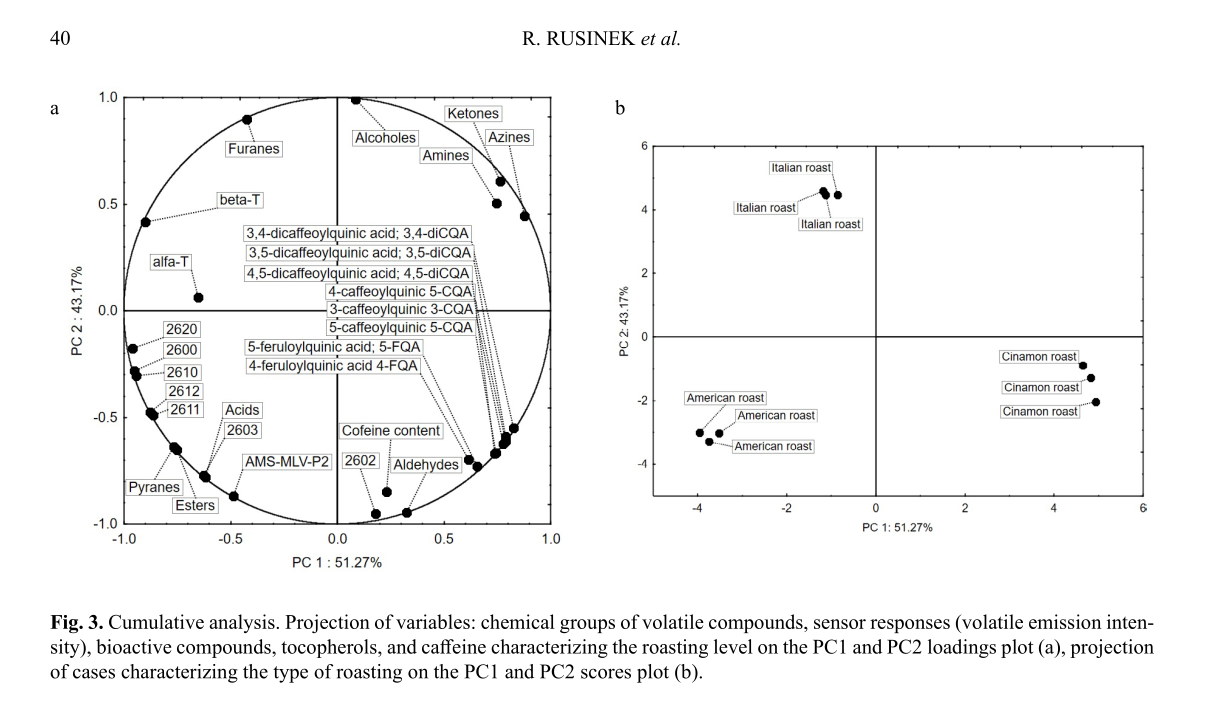
\includegraphics[width=0.9\textwidth]{images/roasted.png}
	\caption*{Análisis de componentes principales (PCA) aplicado al café Arábica. 
		(a) Proyección de variables: compuestos volátiles (furanos, alcoholes, aldehídos, ácidos, piranos y ésteres), compuestos bioactivos (ácidos clorogénicos, tocoferoles y cafeína) y respuestas de sensores. 
		(b) Distribución de los tres niveles de tostado (Cinnamon, American e Italian roast) sobre los ejes PC1 y PC2, mostrando la separación según el perfil químico y aromático.}
	\label{fig:pca_coffee}
	\label{fig:ajuste-gaussiano}
\end{figure} \vspace{0.5cm}

\textbf{Enlace}: \href{https://agro.icm.edu.pl/agro/element/bwmeta1.element.agro-8af7216c-f90d-44af-aaf1-0ffaf3c28eec}{International Agrophysics} \vspace{0.5cm}


\subsubsection{\textbf{Artículo 8:} \textcolor{coolgray}{\textbf{Some biochemical compounds in coffee beans and methods developed for their analysis (2011) - International Journal of the Physical Sciences}}} \vspace{0.5cm}

\textbf{Autores}: \textit{Belay, Abebe}; \textit{Ture, Kalkidan}; \textit{Redi, Mesfin}; \textit{Asfaw, Abebe}. \vspace{0.5cm}

\textbf{Resumen}: Este estudio ofrece una \textbf{síntesis amplia sobre los compuestos bioquímicos presentes en los granos de café} y las técnicas que se han desarrollado para analizarlos. El foco principal está en la \underline{cafeína} y los \underline{ácidos clorogénicos (CGAs)}, considerados los dos compuestos más influyentes tanto en la calidad sensorial del café como en sus efectos fisiológicos.  

Se revisan sus propiedades químicas, su papel en el metabolismo de la planta, su impacto en la salud humana y los \textbf{métodos analíticos empleados} para cuantificarlos, comparando ventajas y limitaciones. El objetivo es aportar un panorama actualizado sobre cómo estos compuestos determinan el valor del café en la industria alimentaria y farmacéutica. \vspace{0.5cm}

\textbf{Resultados}:  
\begin{itemize}
	\item \underline{\textbf{Cafeína}}:
	\begin{itemize}
		\item Es el \textbf{alcaloide principal} en el café (fórmula química: $C_{8}H_{10}N_{4}O_{2}$). Presente en mayor proporción en \textit{C. canephora} (\textbf{Robusta}) (2.2\% promedio) frente a \textit{C. arabica} (\textbf{Arábica}) (1.2\% promedio).  
		\item Sus niveles dependen principalmente de la \underline{genética de la especie} y no tanto de factores ambientales. El tostado apenas modifica su contenido.  
		\item Fisiológicamente, actúa como \textbf{estimulante del sistema nervioso central}, pero en dosis elevadas puede generar efectos adversos: insomnio, taquicardia o disfunciones renales.  
		\item Está vinculada a la \textbf{calidad del café}: un contenido más alto suele asociarse a cafés de menor calidad.  
		\item \textbf{Métodos de análisis}: espectrofotometría UV-Vis, HPLC (el más confiable), FTIR, NIR y electroforesis capilar. El HPLC destaca por su precisión, aunque es costoso.  
	\end{itemize}
	
	\item \underline{\textbf{Ácidos Clorogénicos (CGAs)}}:
	\begin{itemize}
		\item Son los \textbf{principales compuestos fenólicos} en granos de café verde, especialmente los \textbf{ácidos cafeoilquínicos (CQAs)} y sus isómeros.  
		\item Su contenido varía: en \textit{C. arabica} (4–8.4\%) y en \textit{C. canephora} (7–14.4\%).  
		\item Tienen un rol fundamental como \textbf{antioxidantes}, con propiedades \underline{anticancerígenas, antiinflamatorias} \underline{y antihipertensivas}. También se han vinculado con la reducción del riesgo de diabetes tipo 2.  
		\item En la planta, contribuyen a la \textbf{resistencia contra plagas y enfermedades}. En la bebida, determinan la \textbf{acidez, amargor y formación de aroma} a través de reacciones de Maillard y Strecker.  
		\item \textbf{Métodos de análisis}: HPLC, electroforesis capilar y espectroscopía (UV-Vis, fluorescencia). Aunque precisos, suelen ser lentos y requieren instrumentación cara.  
	\end{itemize}
\end{itemize} \vspace{0.5cm}

El estudio resalta que tanto la \textbf{cafeína} como los \textbf{ácidos clorogénicos} no solo son determinantes en la \underline{calidad} \underline{sensorial del café}, sino que también poseen un gran interés en el campo de la salud y en el desarrollo de productos nutracéuticos. Tambień se enfatiza en la necesidad de seguir perfeccionando \textbf{métodos de análisis más rápidos y accesibles} para su monitoreo en la industria cafetera. \vspace{0.5cm}

\textbf{Enlace}: \href{https://www.researchgate.net/profile/Abebe-Gemta/publication/228467568_Some_biochemical_compounds_in_coffee_beans_and_methods_developed_for_their_analysis/links/65a79b2a47fc9041629d70c2/Some-biochemical-compounds-in-coffee-beans-and-methods-developed-for-their-analysis.pdf}{Researchgate} \vspace{0.5cm}

\subsubsection{\textbf{Artículo 9:} \textcolor{Cavern Pink}{\textbf{The influence of brewing method on bioactive compounds residues in spent coffee grounds of different roasting degree and geographical origin (2019) - International Journal of Food Science and Technology}}} \vspace{0.5cm}

\textbf{Autores}: \textit{Głowacka, R.}; \textit{Górska, A.}; \textit{Wirkowska-Wojdyła, M.}; \textit{Wosiak, R.}; \textit{Majewska, E.}; \textit{Derewiaka, D.} \vspace{0.5cm}

\textbf{Resumen}: Este estudio examinó la influencia del \textbf{método de preparación de café} (Moka, filtrado, goteo e infusión), el \underline{grado de tueste} (claro y oscuro) y el \underline{origen geográfico} (Nicaragua, Colombia y México) sobre el contenido de \textbf{compuestos bioactivos en los residuos de café molido usado (Spent Coffee Grounds, SCG)}.  

El propósito fue evaluar el potencial de los SCG como fuente de compuestos funcionales (cafeína, ácidos clorogénicos y polifenoles), en el marco de la \textbf{economía circular} y la valorización de subproductos alimentarios. Además, se analizaron parámetros relacionados con la \textbf{actividad antioxidante} y el \textbf{índice de pardeamiento}, ambos vinculados a compuestos fenólicos y melanoidinas. \vspace{0.5cm}

\textbf{Resultados}:  
\begin{itemize}
	\item \underline{\textbf{Cafeína}}:  
	El contenido en SCG varió de 2.94 a 13.19 mg g$^{-1}$ dm, siendo más alto en cafés \textbf{filtrados}, ya que este método extrae menos cafeína hacia la bebida. El menor contenido se registró en cafés preparados con cafetera Moka.  
	
	\item \underline{\textbf{Ácidos clorogénicos (CGAs)}}:  
	Se detectaron 3-CQA, 4-CQA, 5-CQA y di-CQAs en todos los SCG. El \textbf{ácido 3-CQA fue el predominante}. Los residuos de cafés de \textbf{tueste claro conservaron más CGAs} que los de tueste oscuro, confirmando que el calor degrada estos compuestos. Los SCG de café filtrado fueron los más ricos en CGAs, con valores de hasta 13.28 mg g$^{-1}$.  
	
	\item \underline{\textbf{Índice de pardeamiento}}:  
	Más alto en SCG de \textbf{tueste oscuro}, con incrementos del 48–76\% respecto a los de tueste claro. El método de infusión produjo los valores más bajos.  
	
	\item \underline{\textbf{Polifenoles totales (TPC)}}:  
	El contenido osciló entre 25.13 y 46.23 mg g$^{-1}$. Los SCG de \textbf{café oscuro por goteo} tuvieron los valores más altos. Estos niveles superan los reportados en frutas ricas en antioxidantes como moras y frambuesas.  
	
	\item \underline{\textbf{Actividad antioxidante (AA)}}:  
	Se encontró entre 45.06 y 113.61 mg Trolox g$^{-1}$ SCG. La mayor actividad se registró en cafés de \textbf{filtrado y goteo}, así como en SCG de \textbf{tueste oscuro}, posiblemente debido a la formación de melanoidinas.  
\end{itemize} \vspace{0.5cm}

Los \textbf{residuos de café} aún conservan cantidades significativas de \underline{cafeína, polifenoles y compuestos antioxidantes}, especialmente cuando provienen de métodos de filtrado o goteo. Esto los convierte en una \textbf{fuente infrautilizada de compuestos bioactivos} con potencial aplicación en la industria alimentaria, farmacéutica y cosmética. Se recomienda desarrollar técnicas de extracción más seguras (alternativas al metanol) para su aprovechamiento industrial. \vspace{0.5cm}

\textbf{Enlace}: \href{https://academic.oup.com/ijfst/article/54/11/3008/7805223}{Oxford Academic} \vspace{0.5cm}


\subsubsection{\textbf{Artículo 10:} \textcolor{pakistangreen}{\textbf{Relationship between physico-chemical properties in the coffee beans and the cup quality attributes of coffee from the state of Chiapas, Mexico (2020) - International Food Research Journal }}} \vspace{0.5cm}

\textbf{Autores}: \textit{Cortés, F. M.}; \textit{Pérez, S. J. A.}; \textit{Servín, J. R.}; \textit{Morales, R. V.} \vspace{0.5cm}

\textbf{Resumen}:  \vspace{0.5cm}

Este estudio se centró en evaluar la relación entre las \underline{propiedades fisicoquímicas de los granos de café verde} y los \underline{atributos de calidad en taza}, utilizando 139 muestras recolectadas en las 13 regiones productoras de café del estado de Chiapas, México. La investigación partió de la importancia de Chiapas como principal productor de café del país, responsable de alrededor del 40\% de la producción nacional en 2018, y buscó determinar cómo factores físicos (forma, tamaño, defectos) y químicos (cafeína, trigonelina y ácido clorogénico - 5-CQA) influyen en las características sensoriales del café tostado y catado.  

Las muestras fueron procesadas \textit{in situ} por el método húmedo, analizadas mediante UPLC-QTof (Ultra Performance Liquid Chromatography coupled with Quadrupole Time-of-Flight Mass Spectrometry) para la cuantificación química, y evaluadas sensorialmente por catadores certificados (Q-graders) bajo los protocolos de la \textbf{SCAA}, considerando atributos como aroma, acidez, cuerpo, sabor, regusto, equilibrio, dulzura y puntuación general.  

\textbf{Resultados}: \vspace{0.5cm}  

\begin{enumerate}
	\item \textbf{Propiedades físicas}:
	\begin{itemize}
		\item Predominó el \underline{grano plano} (87.1\%), seguido del caracolillo (8.7\%). La forma no afectó la puntuación total, pero sí influyó en \textbf{aroma} y \textbf{cuerpo}.
		\item El \underline{tamaño} no mostró efectos generales en la calidad, excepto en el \textbf{aroma}, donde granos medianos y pequeños obtuvieron mejores puntuaciones que los grandes.
		\item Los \textbf{defectos} fueron bajos en la mayoría de las regiones, salvo en una comunidad de Copainalá.
	\end{itemize}
	
	\item \textbf{Composición química}:
	\begin{itemize}
		\item La \textbf{cafeína} presentó un promedio de 1.7 $\pm$ 0.5\%, por encima del rango típico para \textit{C. arabica}. Su concentración tuvo correlación \underline{negativa} con todos los atributos sensoriales. Cada 100 m de altitud redujo un 0.02\% su contenido.
		\item La \textbf{trigonelina} (1.2 $\pm$ 0.3\%) también mostró correlación \underline{negativa} con la calidad en taza, sin relación con la altitud.
		\item El \textbf{ácido clorogénico (5-CQA)} (4.0 $\pm$ 1.2\%) se correlacionó \underline{positivamente} con los atributos, mejorando en particular la \textbf{acidez}. La altitud favoreció su incremento.
	\end{itemize}
	
	\item \textbf{Evaluación sensorial}:
	\begin{itemize}
		\item El aumento de 100 m en altitud se tradujo en +0.32 puntos en la puntuación total.
		\item La \textbf{acidez} fue el factor más influyente en la calidad total (r = 0.90), seguida del \textbf{equilibrio} (r = 0.88) y la \textbf{apreciación general} (r = 0.88).
		\item El \textbf{sabor} (r = 0.86) y el \textbf{regusto} (r = 0.81) también destacaron como atributos relevantes.
		\item 11 de las 13 regiones alcanzaron $\geq$ 80 puntos en la escala SCAA, clasificando como \textbf{cafés de especialidad}. La región de Bochil obtuvo la mayor puntuación (84.6 $\pm$ 3.9).
		\item Se detectó correlación positiva entre la \textbf{humedad de los granos} y la puntuación total (r = 0.2504).
	\end{itemize}
\end{enumerate} \vspace{0.3cm}

Las propiedades físicas y químicas de los granos, junto con factores ambientales como la altitud, \underline{modulan de manera} \underline{significativa la calidad sensorial del café de Chiapas}, consolidándolo como un origen de alta calidad para la producción de café de especialidad.  

\textbf{Enlace}: \href{http://www.ifrj.upm.edu.my/27%20(04)%202020/DONE%20-%2018%20-%20IFRJ19993.R1.pdf}{International Food Research Journal} \vspace{0.5cm}


\subsubsection{\textbf{Artículo 11:} \textcolor{Mustard}{\textbf{Physico-elemental analysis of roasted organic coffee beans from Ethiopia, Colombia, Honduras, and Mexico using X-ray micro-computed tomography and external beam particle induced X-ray emission (2019) - Food Chemistry: X }}} \vspace{0.5cm}

\textbf{Autores}: \textit{Karen J. Cloete}; \textit{\v{Z}iga \v{S}mit}; \textit{Roya Minnis{-}Ndimba}; \textit{Primo\v{z} Vavpeti\v{c}}; \textit{Anton du Plessis}; \textit{Stephan G.\ le Roux}; \textit{Primo\v{z} Pelicon}. \vspace{0.5cm}

\textbf{Resumen}: En este artículo se hace un estudio comparativo de \underline{granos de café orgánico tostado} (\textit{C. arabica}) provenientes de Etiopía, Colombia, Honduras y México para evaluar \textbf{perfil elemental}, \textbf{rasgos físicos} y \textbf{microestructura}, y explorar su posible \underline{autenticación geográfica}. Se combinaron: (i) \textbf{microscopía de luz} (masa y dimensiones), (ii) \textbf{microtomografía computarizada de rayos X (micro{-}CT)} no destructiva (porosidad y conectividad), y (iii) \textbf{PIXE de haz externo} (Particle Induced X-ray Emission) para cuantificar elementos $>$ Na con sensibilidad de orden \textbf{$\mu$g g$^{-1}$}, permitiendo además \underline{mapeo elemental en muestras intactas y sin vacío}. El tratamiento estadístico incluyó estadística descriptiva, ANOVA (Tukey HSD), mapas de calor con \textit{clustering} jerárquico y \textbf{LDA} (análisis discriminante lineal). \vspace{0.5cm}

\textbf{Resultados}:  
\begin{itemize}
	\item \underline{\textbf{PIXE (composición elemental)}}:
	\begin{itemize}
		\item Macroelementos detectados: P, S, Cl, K, Ca; microelementos: Ti, Mn, Fe, Cu, Zn, Br, Rb, Sr.
		\item Orden de abundancia media: \textbf{K $>$ S $>$ Ca $>$ P $>$ Cl} (macro) y \textbf{Rb $>$ Fe $>$ Mn $>$ Cu $>$ Sr $>$ Zn} (micro).
		\item \underline{Distribución heterogénea} de K y Fe, con máximos en el endospermo.
		\item \textbf{Tendencias regionales}: México con \underline{Cl} más alto; Etiopía con \underline{S} más alto; Colombia con \underline{Rb} y \underline{Sr} más elevados.
		\item \textbf{Ausencia de metales tóxicos}; se observaron \underline{trazas} de Ti y Br en Etiopía y México.
		\item \textbf{LDA}: sin asociación fuerte composición–región; no obstante, \underline{diferencias sutiles} en micronutrientes (Colombia parcialmente separada).
	\end{itemize}
	
	\item \underline{\textbf{Rasgos físicos (microscopía de luz)}}:
	\begin{itemize}
		\item Los granos de \textbf{México} presentaron \underline{mayor masa}.
		\item Los de \textbf{Honduras} mostraron \underline{mayor anchura}; la anchura difirió significativamente entre las cuatro procedencias.
	\end{itemize}
	
	\item \underline{\textbf{Microestructura (micro{-}CT)}}:
	\begin{itemize}
		\item \textbf{Heterogeneidad} intra e intergrano; distribución general de poros relativamente uniforme pero \underline{baja homogeneidad} en sus características a través de regiones morfológicas.
		\item \textbf{Porosidad} (ascendente): Honduras (23.5\%), México (25.23\%), Colombia (30.42\%), \textbf{Etiopía} (31.43\%, con \underline{mayor interconectividad}).
		\item Implicaciones: más conectividad puede \underline{facilitar la molienda} pero \underline{acortar la vida útil} por mayor permeabilidad.
	\end{itemize}
\end{itemize} \vspace{0.2cm}

El enfoque \textbf{multidimensional} (PIXE + micro{-}CT + microscopía) es \underline{viable} para caracterizar café tostado desde la perspectiva \textbf{nutricional} y \textbf{microestructural}. Aunque no se logró una clasificación geográfica robusta con LDA, las \underline{variaciones elementales y físicas} observadas \textbf{tipifican atributos de calidad y almacenamiento} relevantes por región. \vspace{0.5cm}

\textbf{Enlace}: \href{https://www.sciencedirect.com/science/article/pii/S2590157519300343}{ScienceDirect} \vspace{0.5cm}


\subsubsection{\textbf{Artículo 12:} \textcolor{Lemon Ginger}{\textbf{Relationship Between Altitude and Physical, Chemical and Organoleptic Quality Attributes in Beans of \textit{Coffea arabica} L. with Denomination of Origin ``Pluma'' from Oaxaca, Mexico (2024) - Ciencia Latina Revista científica Multidisciplinar}}}
\vspace{0.5cm}

\textbf{Autores}: \textit{Jiménez Mendoza, J.\ A.}; \textit{Santos Sánchez, N.\ F.}; \textit{García Montalvo, I.\ A.}; \textit{Cruz, A.\ M.}; \textit{Varapizuela Sánchez, C.\ F.} \vspace{0.5cm}

\textbf{Resumen}: El café con denominación de origen ``Pluma'' (Oaxaca, México) es reconocido por su \underline{calidad física,} \underline{química y organoléptica}. Este estudio analizó granos de \textit{Coffea arabica} L. de tueste medio, cultivados en tres fincas a diferentes altitudes: \textbf{La Virginia (1058 msnm)}, \textbf{La Palma (1149 msnm)} y \textbf{Nuestra Señora del Carmen (1343 msnm)}. Se evaluaron atributos físicos según la NOM-255-SE-2022, composición química (pH, acidez titulable, humedad, cenizas, lípidos y proteínas) y calidad sensorial mediante catación profesional (Q-Graders, protocolo \textbf{SCA}). El análisis estadístico incluyó \textbf{ANOVA}, pruebas \textbf{Tukey HSD} y \textbf{PCA (Análisis de Componentes Principales)}. \vspace{0.5cm}

\textbf{Resultados}:  
\begin{itemize}
	\item \underline{\textbf{Análisis físico}}:  
	Diferencias significativas en expansión, color, granos claros al tueste y fisura (excepto textura).  
	\textbf{La Virginia}: mayor expansión (95.33$\pm$0.01\%).  
	-\textbf{Nuestra Señora del Carmen}: mayor proporción de granos claros (98.67$\pm$0.01\%), clasificados como calidad \textbf{``premium''}.
	
	\item \underline{\textbf{Análisis químico}}:  
	 \textbf{Acidez titulable}: aumentó con la altitud; mayor en \textbf{Nuestra Señora del Carmen} (23.14$\pm$0.82 mg ácido clorogénico/g).  
	 \textbf{Lípidos}: valores más altos en altitudes mayores (14.23\% en ``Nuestra Señora del Carmen'' vs.\ 13.37\% en ``La Virginia''), asociados al \textbf{cuerpo} de la bebida.  
	\textbf{Proteínas}: aumentaron con la altitud (8.50–8.85\%), dentro del rango reportado para \textit{C. arabica}.  
	 Humedad y cenizas dentro de límites de la norma mexicana.
	
	\item \underline{\textbf{Evaluación organoléptica}}:  
	Todas las muestras clasificadas como \textbf{cafés de especialidad ``premium''}.  
	Puntuaciones: \textbf{La Virginia}: 82.75 pts (máximos en aroma, sabor, regusto, apreciación general).  
	\textbf{Nuestra Señora del Carmen}: 82.75 pts (mejor acidez y cuerpo).  
	 \textbf{La Palma}: 81.85 pts.  
	Descriptores comunes: \textit{chocolate, frutos secos, caña de azúcar y notas limpias}.
	
	\item \underline{\textbf{PCA (Componentes principales)}}:  
	 Explicó el 97.609\% de la varianza total.  
	Correlación positiva fuerte entre \textbf{altitud–proteínas–lípidos–acidez titulable}.  
	Relación inversa entre altitud y textura.  
	Confirmó influencia de variables químicas en la calidad organoléptica.
\end{itemize} \vspace{0.3cm}

La \underline{altitud influye significativamente} en los \textbf{atributos fisicoquímicos y organolépticos} de los granos de café ``Pluma''. Un mayor contenido de lípidos, proteínas y acidez titulable en altitudes elevadas potencia el cuerpo y la acidez de la bebida, consolidando su clasificación como café de especialidad ``premium''. \vspace{0.5cm}

\textbf{Enlace}: \href{https://ciencialatina.org/index.php/cienciala/article/view/15987}{Ciencia Latina Revista Multidisciplinar} 


\href{https://drive.google.com/file/d/1hA02atl50Ln51g2URjeCjpUj-LieqEYm/view?usp=sharing}{Enlace del vídeo de búsqueda de artículos}







\end{document}